\documentclass[tikz,border=2pt,11pt]{standalone}
\usetikzlibrary{calc}
\usetikzlibrary{positioning}
\usetikzlibrary{decorations.pathmorphing}
\usetikzlibrary{arrows.meta}
\usetikzlibrary{fit}
\usepackage{amsmath}
\usepackage{amssymb}
\usepackage{mathrsfs}
\usepackage{graphicx}
\usepackage{xcolor}
\usepackage{tikz}
\newcommand{\C}{\mathbb C}
\newcommand{\Z}{\mathbb Z}
\newcommand{\R}{\mathbb R}
\newcommand{\Q}{\mathbb Q}
\newcommand{\F}{\mathbb F}
\DeclareMathOperator{\tr}{tr}
\DeclareMathOperator{\Ad}{Ad}
\DeclareMathOperator{\End}{End}
\DeclareMathOperator{\Hom}{Hom}
\DeclareMathOperator{\im}{im}
\DeclareMathOperator{\rank}{rank}
\DeclareMathOperator{\SL}{SL}
\DeclareMathOperator{\Spec}{Spec}
\DeclareMathOperator{\Res}{Res}
\DeclareMathOperator{\id}{id}
\begin{document}
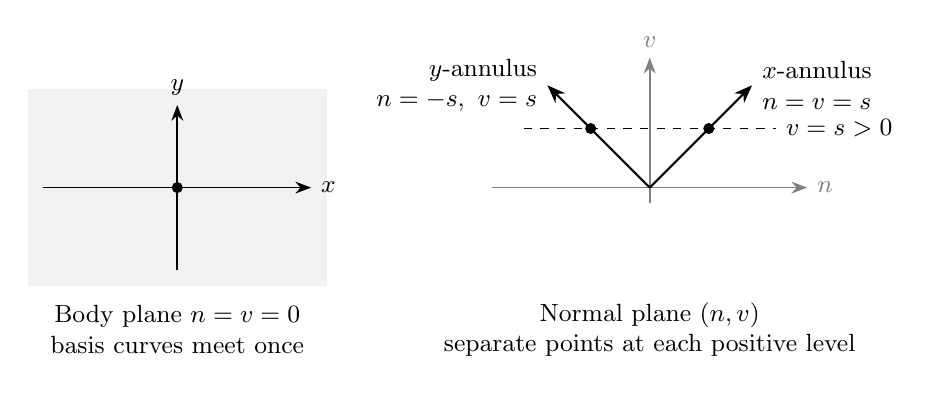
\begin{tikzpicture}[font=\small,>=Stealth,
  every path/.style={line width=.6pt}]
  \begin{scope}[shift={(0,0)}]
    \fill[gray!10] (-1.9,-1.25) rectangle (1.9,1.25);
    \draw[->] (-1.7,0) -- (1.7,0) node[right] {$x$};
    \draw[->] (0,-1.05) -- (0,1.05) node[above] {$y$};
    \fill (0,0) circle (2pt);
    \node[align=center] at (0,-1.8)
      {Body plane $n=v=0$\\basis curves meet once};
  \end{scope}
  \begin{scope}[shift={(6,0)}]
    \draw[->,gray] (-2,0) -- (2,0) node[right] {$n$};
    \draw[->,gray] (0,-.2) -- (0,1.65) node[above] {$v$};
    \draw[->,thick] (0,0) -- (1.3,1.3)
      node[right,align=left] {$x$-annulus\\$n=v=s$};
    \draw[->,thick] (0,0) -- (-1.3,1.3)
      node[left,align=right] {$y$-annulus\\$n=-s,\ v=s$};
    \draw[dashed] (-1.6,.75) -- (1.6,.75);
    \fill (-.75,.75) circle (2pt);
    \fill (.75,.75) circle (2pt);
    \node[anchor=west,inner sep=2pt] at (1.65,.75) {$v=s>0$};
    \node[align=center] at (0,-1.8)
      {Normal plane $(n,v)$\\separate points at each positive level};
  \end{scope}
\end{tikzpicture}
\end{document}
